\documentclass{ximera}
\input{../../preamble}

\addPrintStyle{../..}

\begin{document}
	\author{Bart Lambregs}
	\xmtitle{Bewerkingen met vectoren}{}
    \xmsource\xmuitleg


% SCALAIRE VERMENIGVULDIGING 

% ph: maar met 1 shift vector doen; is veel simpelen -1*(Shift) is de andere
%  TIKZPICTURE DIE DE SCALAIRE VERMENIGVULDIGING ILLUSTREERT 

\subsection*{Scalaire vermenigvuldiging van een reëel getal met een vector}

Wanneer een reëel getal met een vector vermenigvuldigd wordt, dan is er een herschaling van de vector met behoud van richting. 
De grootte en zin kunnen veranderen. Het is een soort reëel veelvoud van de vector. 
De scalarie verminigvuldiging wordt genoteerd als \(\vec{c} = k \cdot \vec{a}\) waarbij \(k \in \R\).

\begin{image}[0.2\textwidth]
\begin{tikzpicture}
    % \draw (-4,-4) grid (4,4);

    \pgfmathsetmacro{\ax}{2}  
    \pgfmathsetmacro{\ay}{0.5}  

    % \pgfmathsetmacro{\c}{$\sqrt{2}$}  
    \pgfmathsetmacro{\d}{2} 

    \coordinate (O) at (0,0); 
    \coordinate (A) at (\ax,\ay); 
    
    \coordinate (Shift) at (0,0.1); 

    \fill (O) circle (2pt); %node[below left]{O};

    \draw[->, very thick,  -latex] (O) -- ($(A)$) node[midway, below]{\(\vec{a}\)};
    \draw[->, very thick,  -latex, blue] ($ (O) - (Shift)$) -- ($-1*(A) - (Shift)$) node[midway, above]{\(-\vec{a}\)};

    \draw[->, very thick,  -latex] ($ (O) + (Shift)$) -- ($\d*(A) + (Shift)$) node[midway, above]{\(2 \cdot \vec{a}\)};
    \draw[->, very thick,  -latex, blue] ($ (O) - 2*(Shift)$) -- ($-0.5*(A) - 2*(Shift)$) node[midway, below]{\(-\frac{1}{2}\vec{a}\)};

\end{tikzpicture}
\end{image}


\subsection*{Samenstelling of som van twee (of meer) vectoren}

Wanneer vectoren van dezelfde grootheid worden opgeteld, bekomt men een nieuwe vector die het netto resultaat is van de samenstelling van de gegeven vectoren. 
Men noemt dit resultaat daarom ook de resultante. Grafisch (kwalitatief) bekomt men de resultante via de kopstaartmethode of parallellogrammethode. 

\begin{image}[0.2\textwidth]
    \begin{tikzpicture}
     % TIKZPICTURE DIE DE SOM VAN TWEE VECTOREN BEREKENT 
    % \draw (-4,-4) grid (4,4);

    \pgfmathsetmacro{\ax}{1}  
    \pgfmathsetmacro{\ay}{2}  
    \pgfmathsetmacro{\bx}{3}  
    \pgfmathsetmacro{\by}{1} 

    \coordinate (O) at (0,0); 
    \coordinate (A) at (\ax,\ay); 
    \coordinate (B) at (\bx,\by); 

    \fill (O) circle (2pt) node[below left]{O};
    % \fill (A) circle (2pt);
    % \fill (B) circle (2pt);

    \draw[->, -latex] (O) -- (A) node[midway, below]{\(\vec{a}\)};
    \draw[->, -latex] (O) -- (B) node[midway, below]{\(\vec{b}\)};
    
    \draw[->, -latex, red, thick] (O) -- ($ (A) + (B)$) node[midway, below]{\(\vec{a} + \vec{b}\)};
    \draw[->, dashed, -latex, red, thick] (A) -- ($ (A) + (B)$) node[midway, below]{\( \vec{b} \)};
    \draw[->, dashed, -latex, red, thick] (B) -- ($ (A) + (B)$) node[midway, below]{\( \vec{a} \)};

\end{tikzpicture}
\end{image}
\captionof{figure}{De optelling van twee vectoren}


De grootte van de resultante bepalen (kwantitatief) kan op verschillende manieren gebeuren, belangrijkste is de meetkundige samenstelling in het oog te houden en zeker niet blindelings de groottes van de gegeven vectoren optellen! 
In evenwijdige of loodrechte gevallen zijn er efficiënte manieren om de resultante te bepalen (som/verschil of stelling van Pythagoras), de meest algemene methode is echter met de (gewijzigde) cosinusregel:

\[
\vec{c} = \vec{a} + \vec{b} \Rightarrow \| \vec{c} \|^2 = \| \vec{c} \|^2 + \| \vec{c} \|^2 + 2 \cdot \|\vec{a}\| \cdot \|\vec{b}\| \cdot \cos(\alpha)
\]

met \(\alpha\) de hoek tussen \(\vec{a}\) en \(\vec{b}\). 

\begin{example}

In onderstaande figuur is \(\|\vec{a}\| = \SI{3}{\newton}\) en \(\|\vec{b}\| = \SI{5}{\newton}\). 
Bijgevolg is  \(\| \vec{c} \| = \|\vec{a}\| + \|\vec{b}\| = \SI{8}{\newton}\). 

\begin{image}[0.2\textwidth]
    \begin{tikzpicture}
        \coordinate (O) at (0,0);
        \coordinate (A) at (1,0);
        \coordinate (B) at (2,0);
        \coordinate (C) at (3,0);

        \coordinate (Shift) at (0,0.05);

        \fill (O) circle (1pt);
        \fill ($ (O) + (Shift) $) circle (1pt);
        \fill ($ (O) - (Shift) $) circle (1pt);


        \draw[->] ($ (O) + (Shift) $)--($ (A) + (Shift) $)  node[midway, above]{$\vec{a}$};
        \draw[->] (O)--(C)                                  node[pos=0.7, above]{$ \vec{c} = \vec{a} + \vec{b} $};
        \draw[->] ($ (O) - (Shift) $)--($ (B) - (Shift) $)  node[midway, below]{$\vec{b}$};
    \end{tikzpicture}
\end{image}
\end{example}

\begin{example}

% hier staat onnauwkeurigheid; de norm moet buiten de bewerking staan; de norm van een verschil is commutatief

In onderstaande figuur is \(\|\vec{a}\| = \SI{3}{\newton}\) en \(\|\vec{b}\| = \SI{5}{\newton}\). 
Bijgevolg is  \(\| \vec{c} \| = \|\vec{a} + \vec{b}\| = \| -3 + 5 \| = \SI{2}{\newton}\). 

\begin{image}[0.2\textwidth]
    \begin{tikzpicture}
        \coordinate (O) at (0,0);
        \coordinate (A) at (-1,0);
        \coordinate (B) at (2,0);
        \coordinate (C) at (1,0);

        \coordinate (Shift) at (0,0.05);

        \fill (O) circle (1pt);
        \fill ($ (O) + (Shift) $) circle (1pt);
        \fill ($ (O) - (Shift) $) circle (1pt);


        \draw[->] ($ (O) + (Shift) $)--($ (A) + (Shift) $)  node[midway, above]{$\vec{a}$};
        \draw[->] (O)--(C)                                  node[pos=0.7, above]{$ \vec{c} = \vec{a} + \vec{b} $};
        \draw[->] ($ (O) - (Shift) $)--($ (B) - (Shift) $)  node[midway, below]{$\vec{b}$};
    \end{tikzpicture}
\end{image}
\end{example}



\begin{example}

In onderstaande figuur is \(\|\vec{a}\| = \SI{3}{\newton}, \; \|\vec{b}\| = \SI{5}{\newton} \text{ en } \alpha = 50^\circ\). 

    \begin{image}[0.7\textwidth]
        \begin{tikzpicture}
            % TIKZPICTURE DIE DE SOM VAN TWEE VECTOREN BEREKENT 
           % \draw (-4,-4) grid (4,4);
       
           \pgfmathsetmacro{\ax}{1}  
           \pgfmathsetmacro{\ay}{2}  
           \pgfmathsetmacro{\bx}{3}  
           \pgfmathsetmacro{\by}{1} 

           \pgfmathsetmacro{\ang}{50} 
       
           \coordinate (O) at (0,0); 
           \coordinate (A) at (\ang :1); 
           \coordinate (B) at (0:1.5); 
           \coordinate (C) at ($ (A) + (B)$); 
           
           \coordinate (Z) at (180:1); 

           \draw[dotted] (O)--(Z);
       
           \draw[->, -latex, blue] (O) -- (A) node[midway, above left]{\(\vec{a}\)};
           \draw[->, -latex, red] (O) -- (B) node[midway, below]{\(\vec{b}\)};
           \draw[->, -latex, green] (O) -- (C) node[pos=1, above right, green]{\(\vec{c} = \vec{a}+\vec{b}\)};
           
           \draw[->, dashed, -latex, red, thick] (A) -- (C) node[midway, above left]{\( \vec{b} \)};
           \draw[->, dashed, -latex, blue, thick] (B) -- (C) node[midway, below right]{\( \vec{a} \)};

           \draw pic[ pic text = \(\alpha\), draw, angle radius=0.7cm]{angle= B--O--A};
           \draw pic[ pic text = \(\gamma\), draw, angle radius=0.4cm]{angle= B--O--C};
           \draw pic[ pic text = \(\varphi\), draw, angle radius=0.4cm]{angle= C--B--O};
           \draw pic[ pic text = \(\varphi\), draw, angle radius=0.4cm]{angle= A--O--Z};
       \end{tikzpicture}
    \end{image}
\end{example}

De grootte van de resultante \(\vec{c}\) wordt bepaald met de cosinusregel: 

% Cosinusregel
\[
\|\vec{c}\|^2 = \|\vec{a}\|^2 + \|\vec{b}\|^2 - 2 \,\|\vec{a}\|\,\|\vec{b}\|\cos\varphi
\]
\[
= \|\vec{a}\|^2 + \|\vec{b}\|^2 - 2 \,\|\vec{a}\|\,\|\vec{b}\|\cos(180^\circ - \alpha)
\]
\[
= \|\vec{a}\|^2 + \|\vec{b}\|^2 - 2 \,\|\vec{a}\|\,\|\vec{b}\|(-\cos\alpha)
\]
\[
= \|\vec{a}\|^2 + \|\vec{b}\|^2 + 2 \,\|\vec{a}\|\,\|\vec{b}\|\cos\alpha
\]
\[
= \sqrt{3^2 + 5^2 + 2 \cdot 3 \cdot 5 \cdot \cos 50^\circ} \approx \SI{7.3}{N}. 
\]

\begin{remark}
Als \(\vec{c} = \vec{a} + \vec{b}\) geldt dus \textbf{niet} dat \(\|\vec{c}\| = \|\vec{a}\| + \|\vec{b}\|\).
\end{remark}


De richting van de resultate (d.w.z. de hoek \(\gamma\)) kan bepaald worden met de sinusregel: 

\[
\frac{\sin\gamma}{\|\vec{b}\|} = \frac{\sin\alpha}{\|\vec{c}\|}
\quad\Longrightarrow\quad
\sin\gamma = \frac{\|\vec{b}\|\sin\alpha}{\|\vec{c}\|}
\]
\[
\gamma = \arcsin\!\left(\frac{5\cdot\sin 50^\circ}{7.3}\right) \approx 18^\circ
\]



Indien meer dan twee vectoren worden samengesteld, telt men eerst twee ervan met elkaar op en het resultaat daarvan telt men met de volgende op, enzovoort totdat alle vectoren in de som zitten (zoals ook met de optelling van getallen gebeurt).


\subsection*{Verschil van twee vectoren}

Het verschil van de getallen acht en vijf is gelijk aan drie. 
Drie is dus het getal dat je bij vijf moet optellen om acht te bekomen. 
Op dezelfde manier is het verschil van vectoren \(\vec{a}\) en \(\vec{b}\) gelijk aan de vector \(\vec{c}\) die je bij \(\vec{b}\) moet optellen om \(\vec{a}\) te bekomen.
 \(\vec{c}\)is dus letterlijk het verschil of 'onderscheid' tussen \(\vec{a}\) en \(\vec{b}\). 
 De eenvoudigste manier om (zowel grafisch als rekenkundig) het verschil te bepalen is door van het verschil een som te maken. 
 \[
\vec{c} = \vec{a}-\vec{b} = \vec{a} + (-\vec{b})
 \]

 Om \(\vec{c}\) te vinden moeten \(\vec{a}\) en \(-\vec{b}\) worden samengesteld.

\begin{image}[0.5\textwidth]
    \begin{tikzpicture}
        
        \pgfmathsetmacro{\r}{1}
        \pgfmathsetmacro{\ang}{30}

        \coordinate (O) at (0:0);
        \coordinate (A) at (\ang :0.8\r);
        \coordinate (B) at (0:\r);
        \coordinate (minB) at (180:\r);

        \fill (O) circle (2pt); 

        \draw[->, blue, thick] (O)--(A) node[midway, above left]{$\vec{a}$};
        \draw[->, red, thick] (O)--(B) node[midway, below]{$\vec{b}$};
        \draw[->, green, thick] (B)--(A) node[midway, above right]{$\vec{c}$};
        
        \draw[->, red, thick] (O)--(minB) node[midway, below]{$-\vec{b}$};
        \draw[->, green, thick] (O)--($(A) - (B)$) node[midway, below]{$\vec{c}$};
        
        \draw[dotted] (A)--($(A) - (B)$)--(minB);
    \end{tikzpicture}
    
\end{image}

Grafisch blijkt overigens dat indien \(\vec{a}\) en \(\vec{b}\) in hetzelfde punt aangrijpen, \(\vec{a} - \vec{b}\) gelijk is aan de vector met als aangrijpingspunt het eindpunt van \(\vec{b}\) en als eindpunt het eindpunt van \(\vec{b}\).

\subsection*{De loodrechte ontbinding of projectie van een vector in componenten}


% dit zou iets uitgebreiden moeten via de omgekeerde richting (een vecor is eerder opgebouwd uit zijn componenten)

Het is vaak nuttig en noodzakelijk in vraagstukken om een vector (loodrecht) te ontbinden in componenten. 
Noteer met \(\vec{a}_x\) de component volgens de \(x\)-as en met \(\vec{a}_y\) de component volgens de \(y\)-as. 
Voor elke vector geldt dan 
\[
\vec{a} = \vec{a}_x + \vec{a}_y
\]

De lengte van de componenten volgt rechtstreeks uit de goniometrische getallen: 

\[
\cos(\alpha) = \frac{\| \vec{a}_x \|}{\| \vec{a} \|} \Rightarrow \| \vec{a}_x \| = \|\vec{a}\| \cdot \cos(\alpha)
\]

\[
\sin(\alpha) = \frac{\| \vec{a}_y \|}{\| \vec{a} \|} \Rightarrow \| \vec{a}_y \| = \|\vec{a}\| \cdot \sin(\alpha)
\]

% TIKZPICTURE DIE DE ONTBINDING IN COMPONENTEN WEERGEEFT 
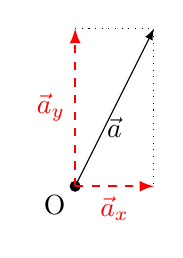
\begin{tikzpicture}
    % \draw (-4,-4) grid (4,4);

    \pgfmathsetmacro{\ax}{1}  
    \pgfmathsetmacro{\ay}{2}  

    \coordinate (O) at (0,0); 
    \coordinate (A) at (\ax,\ay); 

    \fill (O) circle (2pt) node[below left]{O};

    \draw[->, -latex] (O) -- (A) node[midway, below]{\(\vec{a}\)};
    \draw[->, dashed, -latex, red, thick] (O) -- (\ax, 0) node[midway, below]{\( \vec{a}_x \)};
    \draw[->, dashed, -latex, red, thick] (O) -- (0, \ay) node[midway, left]{\( \vec{a}_y \)};

    \draw[dotted] (0,\ay)--(A)--(\ax,0);
        
\end{tikzpicture}

Indien de componenten worden geschreven met behulp van de basisvectoren geeft dit 


$$
\vec{a} = \vec{a}_x + \vec{a}_y = a_x \cdot \vec{e}_x + a_y \cdot \vec{e}_y 
$$


\subsection*{Het scalair product van twee vectoren (of inwendig product)}

Twee vectoren kan men op twee verschillende manieren met elkaar vermenigvuldigen die een ander resultaat opleveren. 

Het scalair product levert een \textbf{scalar} (= getal) als resultaat op die per definitie gelijk is aan de grootte van de projectie van de ene vector op de andere vermenigvuldigd met de grootte van diezelfde andere vector. 

Het scalair product wordt alsvolgt gedefineerd: 

$$
c = \vec{a} \cdot \vec{b} = \| \vec{a}_x \| \cdot \|\vec{b}\| = \|\vec{a}\| \cdot \cos(\alpha) \cdot \|\vec{b}\| = \| \vec{a}\| \cdot \| \vec{b}\| \cdot \cos(\alpha)
$$

% TIKZPICTURE DIE SCALAIR PRODUCT van a op b ILLUSTREERT  
\begin{image}
\begin{tikzpicture}
    % \draw (-4,-4) grid (4,4);

    \pgfmathsetmacro{\ax}{1}  
    \pgfmathsetmacro{\ay}{2}  
    \pgfmathsetmacro{\bx}{3}  
    \pgfmathsetmacro{\by}{0} 

    \coordinate (O) at (0,0); 
    \coordinate (A) at (\ax,\ay); 
    \coordinate (B) at (\bx,\by); 

    \fill (O) circle (2pt) node[below left]{O};
    
    \draw[->, -latex] (O) -- (B) node[midway, below]{$\vec{b}$};

    \draw[->, -latex] (O) -- (A) node[midway, above left]{$\vec{a}$};
    \draw[->, dashed, -latex, red, thick] (O) -- (\ax, 0) node[midway, below]{$ \vec{a}_x $};
    \draw[dashed, -latex, thick] (\ax, 0) -- (A);


    \draw pic[ pic text= $\theta$, draw,  angle radius=0.7cm]{angle = B--O--A}; 
\end{tikzpicture}
\end{image}

\subsection*{Het vectorieel product van twee vectoren (of kruisproduct)}

Het vectorieel product levert een \textbf{vector} als resultaat op waarvan de grootte gelijk is aan de oppervlakte van de parallellogram ingesloten tussen de twee vectoren. 
De richting van het vectorproduct is loodrecht op het vlak gevormd door de twee gegeven vectoren en de zin is te bepalen met de rechterhandregel.

\begin{image}[0.5\textwidth]
    \begin{tikzpicture}
        
        \pgfmathsetmacro{\ax}{0.5}
        \pgfmathsetmacro{\ay}{1}
        \pgfmathsetmacro{\bx}{1}
        \pgfmathsetmacro{\by}{0}

        \coordinate (O) at (0,0);
        \coordinate (A) at (\ax,\ay);
        \coordinate (B) at (\bx,\by);

        \fill[gray] (O)--(A)--($(A)+(B)$)--(B)--cycle;

        \draw[->, -latex, blue] (O)--(A) node[midway, above left]{$\vec{a}$};
        \draw[->, -latex, red] (O)--(B) node[midway, below]{$\vec{b}$};

        \draw[dotted] (\ax,0)--(A) node[midway, right]{$\|\vec{a}_y\|$};

        \fill (O) node[]{\(\otimes\)};


    \end{tikzpicture}
\end{image}


\end{document}
